\section{Experimental setup}\label{sec:setup}

The experimental setup is depicted in \cref{fig:setup}. The setup is driven by a modelocked Ti:sapphire laser. The laser emits femtosecond pulses at a wavelength of \qty{810}{\nm}, with a repletion rate of \qty{80}{\MHz} and an average output power of \qty{4}{\W}. The laser beam then passes through an optical parametric oscillator (OPO), where the beam undergoes nonlinear frequency conversion resulting in two outputs: an idler wave and a signal wave. The OPO idler wave can be tuned from \qtyrange{1.7}{4}{\um} and has a maximum output power of \qty{650}{\mW}. The idler has been tuned to a specific wavelength of \qty{2071.7}{\nm} and was stabilized using an integrated automated feedback loop.

To further achieve a wide range of pulse fluences, the laser beam is directed through two wire-grid polarizers. One of the polarizers is placed on a controllable rotation stage to adjust the beam attenuation. The wire-grid polarizers have a broad range of attenuation across different wavelengths and do not alter the beam path during rotation. After the attenuation stage, the beam passes through a beamsplitter, which separates it into two arms: the reference arm and the sample arm. 

The reference arm contains a highly-reflective mirror of known reflectivity from which the leaking signal is collected in a photodiode to monitor the fluence during a measurement. 
The VECSEL chip is placed at the end of the sample arm. Before the beam is incident on the VECSEL, a focusing lens is used to achieve higher fluences on the VECSEL. The VECSEL is probed under normal incidence angle, and its reflection is collected using the same lens. Both beams are recombined at the beamsplitter and directed to an integrating sphere photodiode to measure the total reflected power. The pump beam shines on the VECSEL at a \qty{30}{\degree} angle and is shown in green. 

To measure the different signals from the two different arms and also measure the photoluminescence (PL) signal of the pumped VECSEL chips, two choppers are used. The two choppers separate the signals in time allowing to measure the signals with the same detector. The choppers are phase locked and chopper 2 is run at half of the frequency of chopper 1, specifically at \qty{55}{\Hz}. Chopper 2 is placed in the beam path before the attenuator to block the beam during every second cycle of chopper 1. This allows to isolate the PL signal. Chopper 1 is placed such that both arms can be intercepted by the blades, enabling the passage of light from both or either of the arms. During one cycle of chopper 2, five distinct state can occur, each allowing for a different measurement configuration:
\begin{enumerate}
    \item Only the sample signal, composed of the photoluminescence and the sample signal (S+PL)
    \item Both arms are open, allowing the combined signal from the sample and reference arm  (S+PL+M)
    \item Only the reference signal (M)
    \item Both arms are blocked and only the background signal from the detector is measured (Z)
    \item The probe beam gets blocked and only the (PL) signal is measured
\end{enumerate}

To obtain the reflectivity from the VECSEL, the (PL) and the background signal (Z) are subtracted from the sample signal (S+PL). The resulting value is then compared the reference measurement (M). This yields a scaling factor R, which then can be used to calculate the reflectivity based on the known reflectivity of the reference mirror. To obtain accurate measurement point, 200 such signal iteration are averaged for the final measurement point.
\newpage

\begin{figure}[ht]
    \centering
    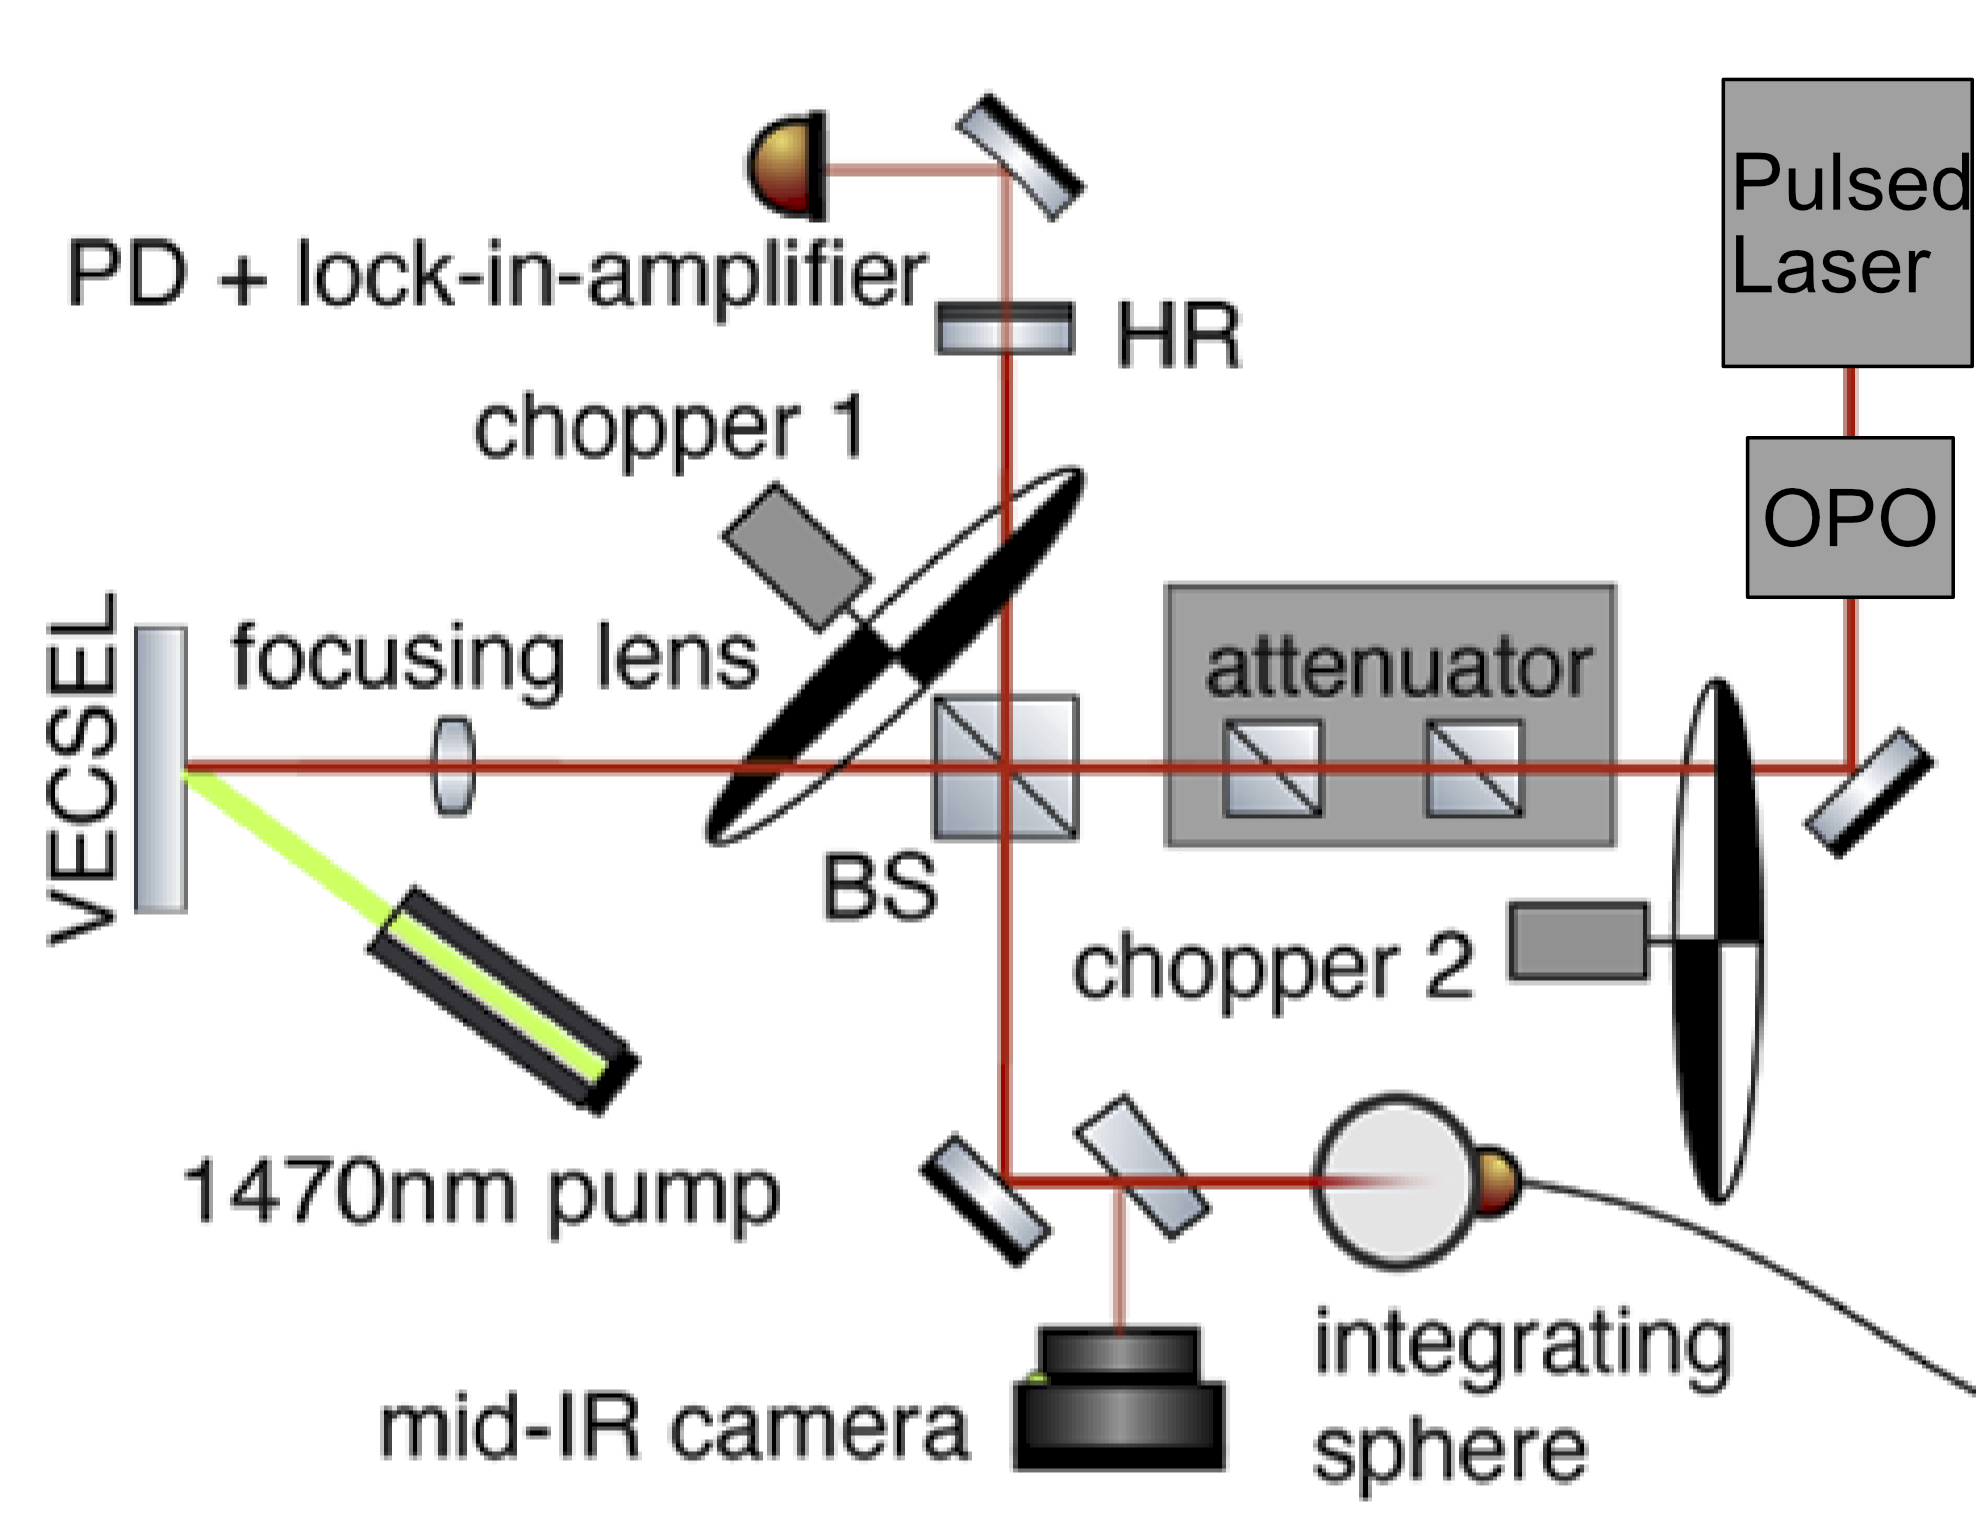
\includegraphics[width=0.8\linewidth]{images/setup.png}
    \caption{On top: Experimental Setup for gain characterization of VECSEL chips. The laser source is a tuneable optical parametric oscillator pumped by a modelocked Ti:sapphire laser. An attenuation stage controls the incident probe fluence on the VECSEL. The pump beam enters the setup at a \qty{30}{\degree} angle. Two choppers, phase-locked and operating at different frequencies, are positioned to differentiate signals and measure photoluminescence (PL) emitted by the pumped VECSEL chip. The figure showcases the key components and their relative positions within the experimental setup.
    On bottom: Visualization of the five different configurations of the two choppers and the measured signal, adjusted from \cite{Mangold2012VECSELCharacterization}.}
    \label{fig:setup}
\end{figure}

\subsection{Automation of the pump power}{\label{subsubsection:pump}}

To improve the time efficiency and increase the unattended measuring time of the experimental setup, the control of the pump power has been automated. In the original setup, the pump power of the laser diode was controlled over a Delta Elektronika SM 18-50 DC power supply, which can deliver up to \qty{50}{\ampere} at up to \qty{18}{\volt}. The power supply was connected over a serial interface controller to a computer and integrated into the already existing user interface of the measurement setup. To implement the control of the pump, a new text field has been added to the user interface where a list of current values for the power supply can be added. Instead of specifying power values directly, the decision was made to enter current values instead due to the potential for enchaining the pump laser diode in the future, which would necessitate to adjust the controller in the software. The software then iterates over this lists and makes a complete measurement for each current value in the list. However, the full automation also required to adjust the signal processing algorithm of the software, which will be discussed in the next section. 

\begin{figure}[ht]
    \centering
    \sidesubfloat[]{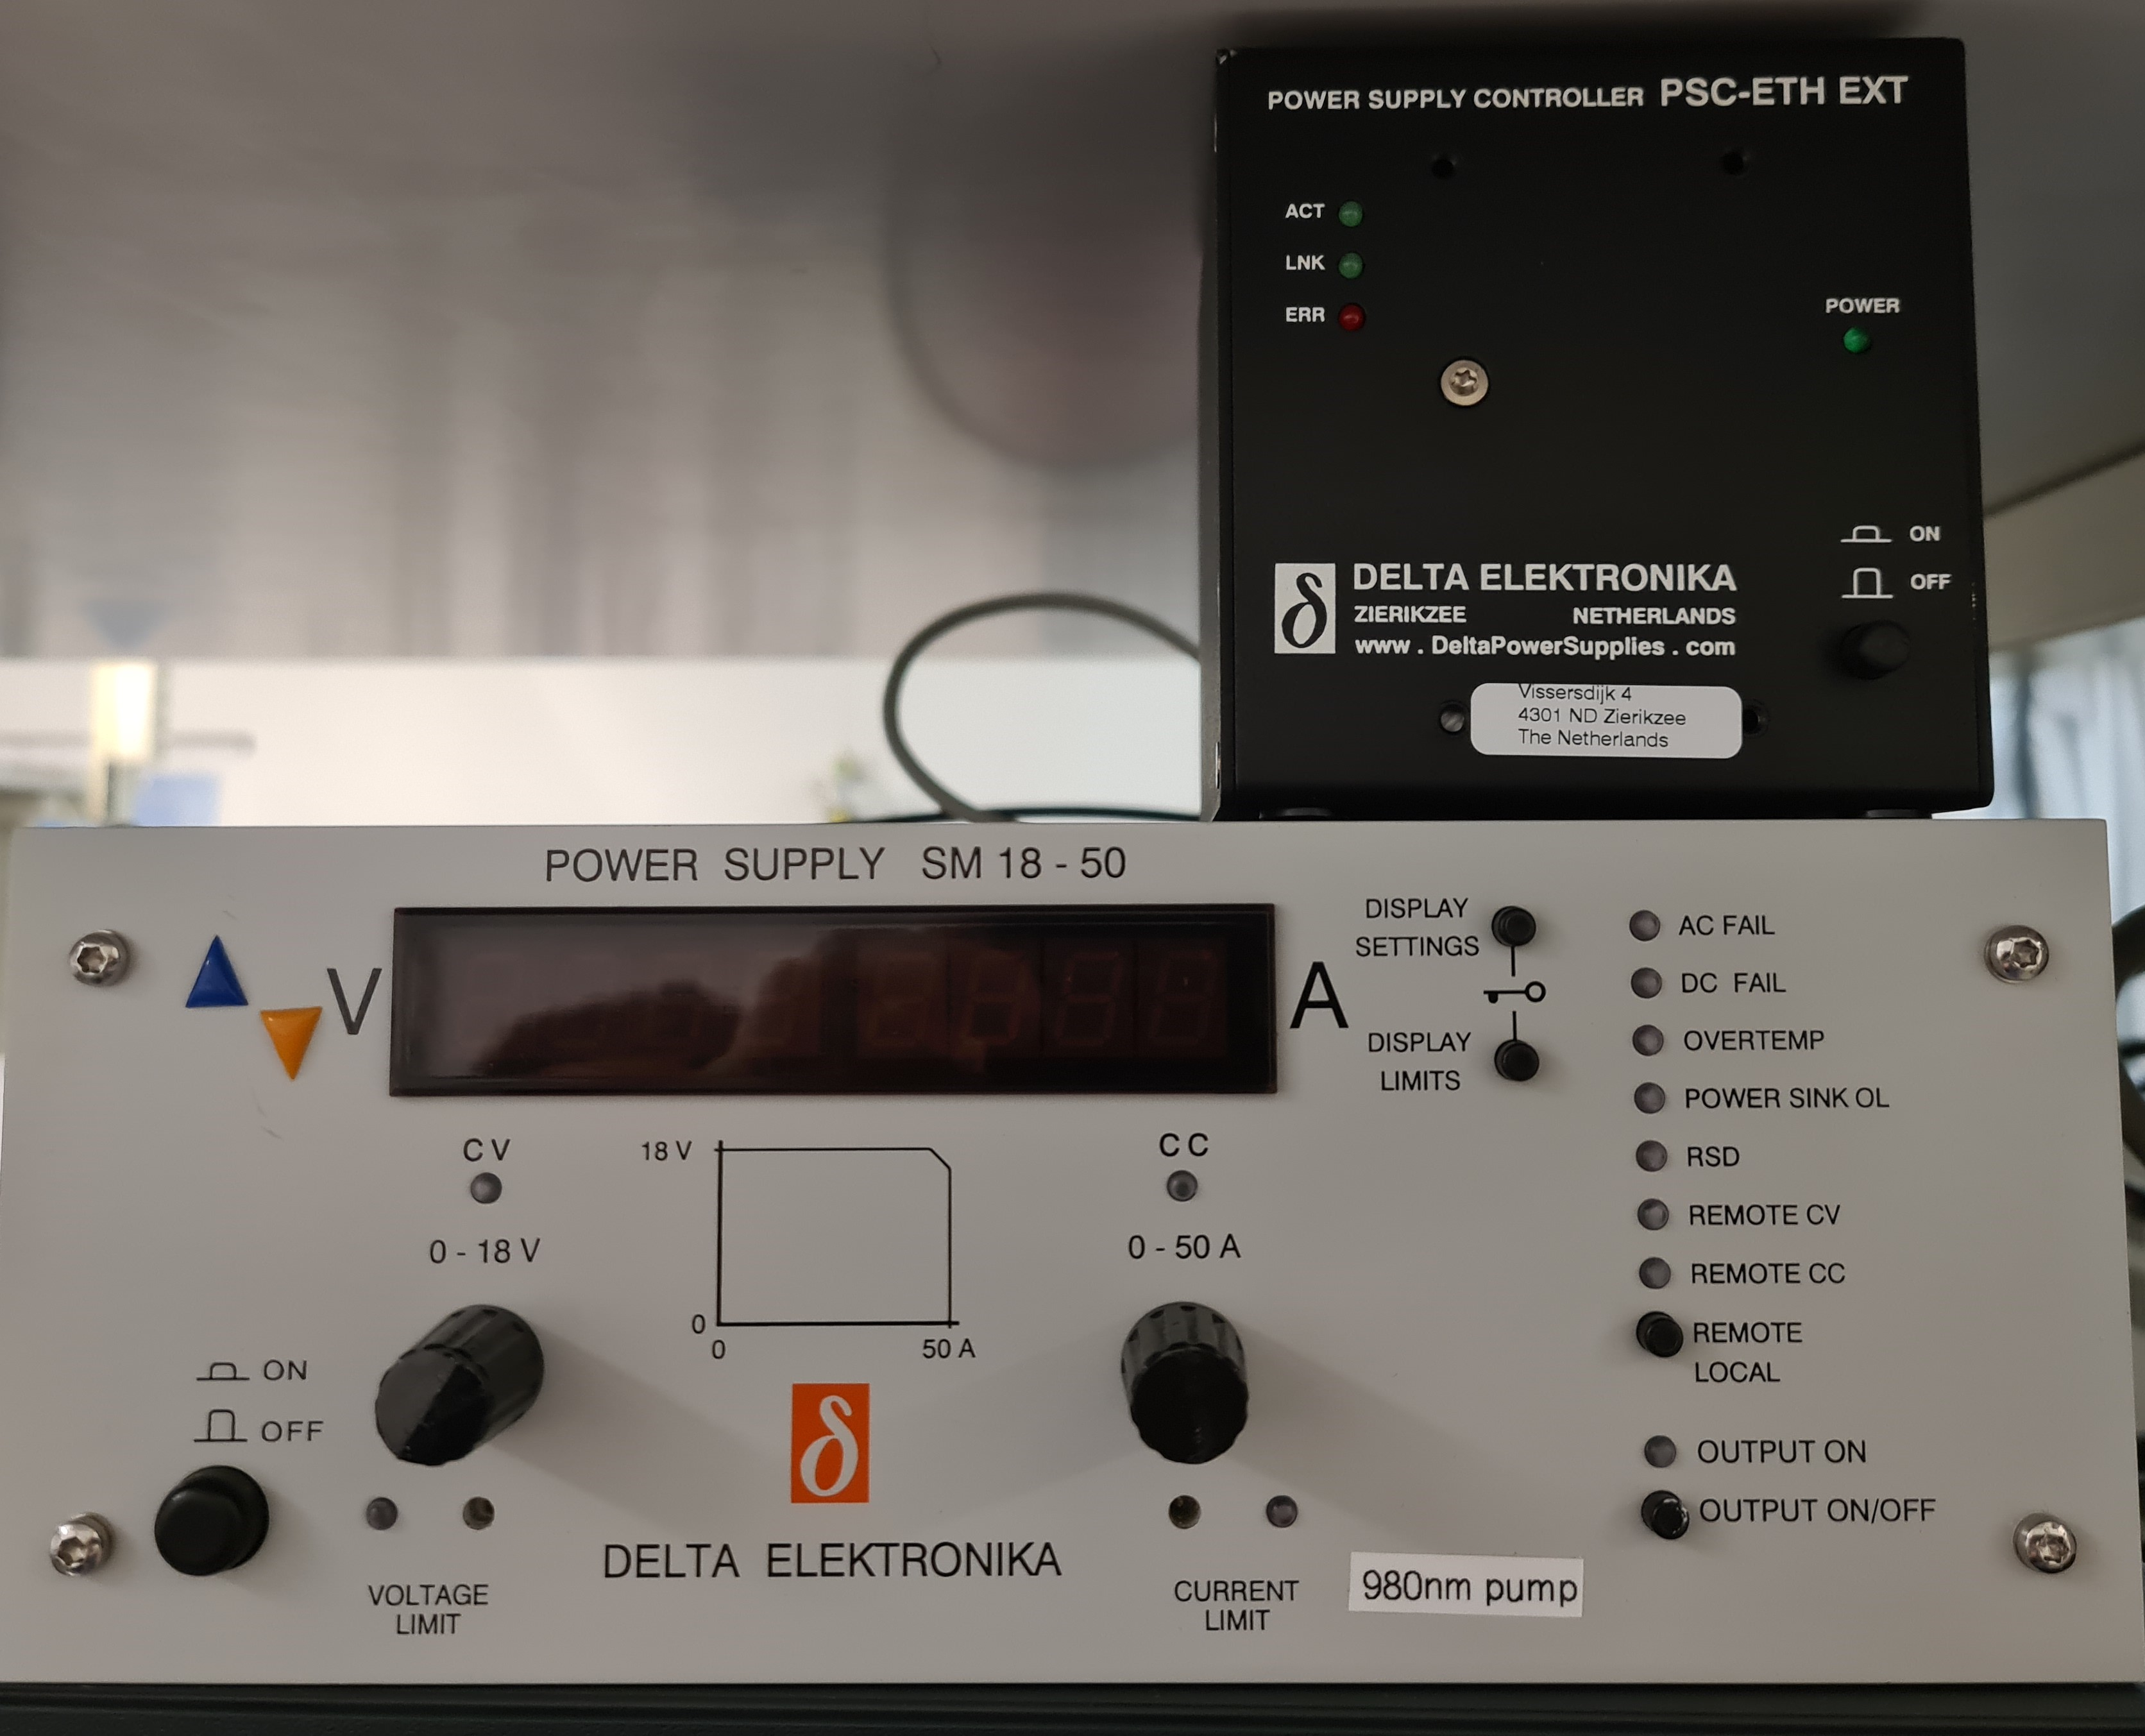
\includegraphics[height=6.5cm]{images/powersupply.jpg}\label{fig:supply}}
    \hfill
    \sidesubfloat[]{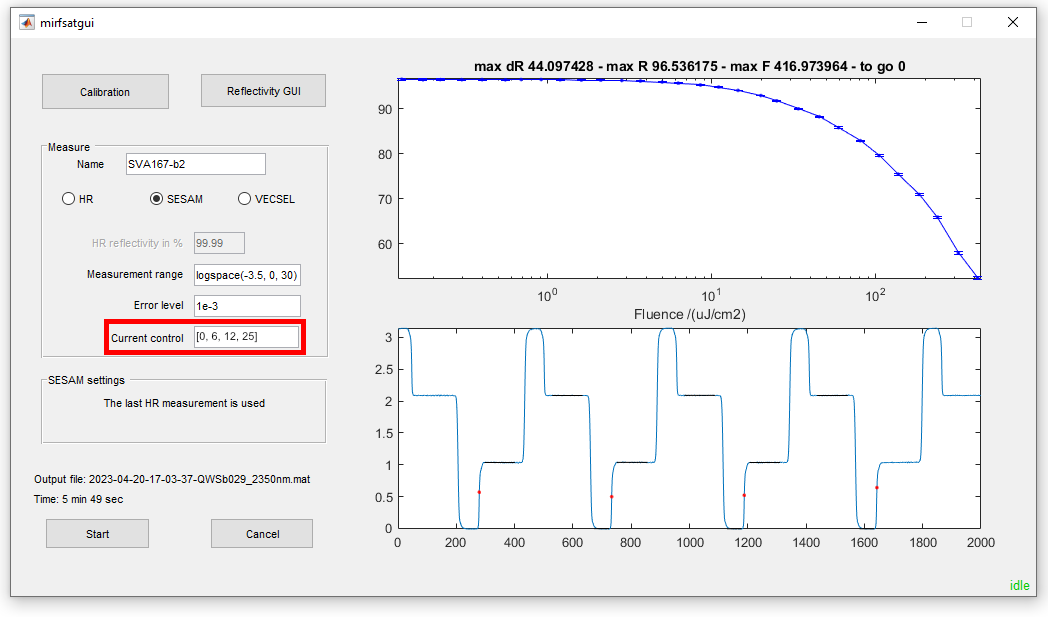
\includegraphics[height=7cm]{images/software.png}\label{fig:software}}
    \caption{a) Image of the Delta Elektronika power supply with the serial interface on top. b) User interface of the measurement setup with the newly added input field for the current control values. }
    \label{fig:auto}
\end{figure}
